\documentclass{article}

\usepackage{corl_2026} % Use this for the initial submission.
\usepackage{xcolor}
% \usepackage[final]{corl_2026} % Uncomment for the camera-ready ``final'' version.
% \usepackage[preprint]{corl_2026} % Uncomment for pre-prints (e.g., arxiv); This is like ``final'', but will remove the CORL footnote.
\usepackage{graphicx}

\newcommand{\YZ}[1]{{\color{blue}#1}}

\title{Self-Labeled Preference Transfer: Bootstrapping Steerable Robot Manipulation on Unlabeled Tasks}



\author{
  Jane E.~Doe\\
  Department of Electrical Engineering and Computer Sciences\\
  University of California Berkeley
  United States\\
  \texttt{janedoe@berkeley.edu}
}


\begin{document}
\maketitle

%===============================================================================

\begin{abstract}
Robot datasets nowadays span across massive tasks, scenes, and objects, but usually only demonstrate a single way to do each task.
However, the same task instruction often admits several acceptable solutions that differ in \emph{how} the task is carried out rather than \emph{what} is achieved; we call these missing axes in the datasets as \emph{preferences}.
Teaching a policy to follow such preferences normally means collecting multi-mode demonstrations and corresponding preference labeling, and this labeling recurs for every new task.
We ask whether preference-following can instead be learned once and transferred, where preferences are densely labeled on a source task set, and a target task set provides the demonstrations only.
However, naive finetuning on all the available training pairs with action loss ties no behavior to the preference, and the steerability from source training can quickly wash out.
To tackle the challenge, we propose \textbf{Self-Labeled Preference Transfer (SPT)}.
In Stage~A, a shared vision-language backbone is trained on the labeled source both to act on a stated preference and to infer the preference of a demonstration.
In Stage~B, the frozen source model labels each unlabeled target demonstration with its inferred preference, and the action policy is then trained on these self-labeled prompts; at test time the user states a preference from the source vocabulary.
Across five preference axes in simulation, the frozen source model labels the unlabeled target with \textbf{96.4\%} accuracy, and SPT raises preference-following by \textbf{25.4} points over a naive finetune (FT) baseline that does not self-label, while task success is essentially unchanged.
On a real UR5e, SPT transfers preference control to two unlabeled target tasks, pushing and billiards, raising preference-following by about \textbf{40} points over the naive FT baseline while keeping task success high.



% In simulation across four preference axes, the source-trained recognizer recovers the correct target preference \textbf{[81]}\% of the time (chance \textbf{[50]}\%), and SPT lifts preference-following by \textbf{[20]} points over a finetune baseline without self-labeling.
% On a UR5e, the same recipe transfers preference control to two task sets it never saw labeled: pick-and-place to pushing, and air-hockey to billiards.
% Finally, we relate when this transfer holds up to how strongly each preference is expressed in motion.
\end{abstract}

\keywords{Preference-Conditioned Policies, Vision-Language-Action Models, Transfer, Imitation Learning}


\section{Introduction}

Robot datasets today span a remarkable range of tasks, scenes, and objects, enabling significant advances in generalist robot policies that condition on language and generalize across embodiments and environments~\cite{o2024open}. Nevertheless, these datasets typically demonstrate only one mode to succeed for each task ~\citep{libero, liberoplus}.
In practice, however, the same instruction often admits multiple acceptable executions: when grasping a mug, one might grasp near its rim or near its base; when placing an item, one might set it down gently or release it from above.
Along these missing axes, which we call \emph{preferences}, today's VLAs react to \emph{what} is asked but not to \emph{how} it should be carried out. The straightforward approach to enabling VLAs to achieve the preference-following capability is to include the multi-mode demonstrations in training.
However, adding such preferences for \emph{every single task} in a dataset is very demanding, as one has to not only collect the corresponding demonstrations, but also label each demonstration with its preference (e.g., by modifying the language description of the task) for building a connection between behavior and the preference prompt.
% Moreover, the same demanding effort for collecting and relabeling are asked again once a new task suite arrives.
% Despite that many existing approaches can supply the relabeling part in various forms ~\citep{zhang2024grape,xia2025hapo, moletta2026rko, ghosh2025prefvlm, singh2025varp}, the labeling effort recurs for every new task, so the policy cannot move beyond instruction following without fresh per-task labels.
% This is particularly costly because the underlying robot datasets already capture rich variation across tasks, scenes, and objects, but they miss the variety of multiple solutions within a single task.


\begin{figure}[t]
  \centering
  \includegraphics[width=\linewidth]{figures/teaser.png}
  \caption{\textbf{Motivation and overview.} One single task can often be completed in multiple valid ways that reflect different user preferences. Existing robot datasets and VLAs primarily learn \emph{what} to accomplish, but not \emph{how} to execute tasks according to user preferences. We propose \textbf{Self-Labeled Preference Transfer (SPT)}, which learns preference-following from densely labeled source tasks and transfers this capability to unseen tasks and objects without requiring preference labels on the target task.}
  \label{fig:teaser}
\end{figure}

In this paper, we show that we do not have to obtain training data with labeled preference for every single task, and instead can make preference-following itself a transferable capability of VLAs---just as modern VLAs transfer understanding of tasks, scenes, and objects to new domains. 
Rather than labeling preferences for every task, we aim to pretrain VLAs with preference-following data \emph{once on a densely-labeled source dataset}.
When deployed on new task sets that include multi-solution demonstrations but with no preference labels, the VLA still inherits steerability through the same preference prompt as the steering handle. 
We call this problem \emph{label-free preference transfer}. 
Since the demonstrations in target tasks offer no preference prompts for training, naively finetuning on the demonstrated trajectories alone provides no signal that ties executed motions to a preference, and the steerability instilled by the source-data pretraining quickly gets forgotten as the policy adapts.

% This reframes the problem from per-task annotation to cross-task transfer: the upfront investment in source labeling amortizes across future tasks, making preference customization as accessible as task generalization.

To solve this problem, we propose \textbf{Self-Labeled Preference Transfer (SPT)}, a two-stage pipeline that couples preference-conditioned acting with preference recognition during source training, and reuses the model's own vision-language backbone to self-label the unlabeled behaviors. Our intuition is that source training on densely labeled preference data does two things at once: it shapes a vision-language representation that lets the action head act on a stated preference, and it teaches the backbone to read the preference from demonstrations. Specifically, \emph{Stage~A} jointly trains a preference-conditioned action head and a preference-recognition head over a shared vision-language backbone on the densely-labeled source;
% This trains the VLA to act on a preference prompt, and due to the addition of the preference-recognition head, also trains the vision-language backbone to understand preferences from demonstrated trajectories alone. 
in \emph{Stage~B}, given the target data without preferences stated in the prompt, the frozen vision-language backbone pseudo-labels the preference for every target demonstration, and the action head is then finetuned on those pseudo-labeled prompts.
% As a result, during deployment, the VLA produces preference-consistent behavior when the user states a preference from the source vocabulary.


% \textbf{preference recognition can explicitly label the prompt and implicitly shape the representation}:
We evaluate SPT in both simulation and real world. Because existing simulation-based manipulation benchmarks vary appearances and initializations but demonstrate a single behavior per task~\citep{libero, liberoplus}, we synthesize preference-varied demonstrations on RoboTwin~\citep{robotwin} across five axes: grasp contact height, release height, obstacle clearance, grasp orientation, and placement location. In the real world, we test with a real UR5e under two cross-task transfer settings: pick-and-place to pushing, air-hockey to billiards.
Across these settings the source-trained recognizer recovers the correct preference on the unlabeled target \textbf{[81]}\% of the time (chance \textbf{[50]}\%), preference-following improves by \textbf{[20]} points over a finetune baseline without self-labeling, and on the UR5e SPT follows the commanded preference on both unlabeled target tasks.

In summary, our contributions are:
(1) We identify execution \emph{preferences}, the multiple valid ways to carry out one task, as a mode of variation that current robot datasets and VLAs leave out.
(2) We formulate \emph{label-free preference transfer}, where preferences are densely labeled on a source task set and must be inherited on a target set with none; to our knowledge, this is the first work to treat execution preference as a cross-task transfer capability of VLAs.
(3) We propose SPT, which co-trains a preference-conditioned action head and a preference-recognition head over a shared vision-language backbone, then reuses that backbone to self-label the target demonstrations, supplying the missing labels without any target annotation.
(4) Across simulation and a real UR5e, SPT achieves preference control on unlabeled tasks, with 96.4\% recognition accuracy and a 25-point gain in preference-following over the no-self-label baseline.


% (1) We identify preference-following as a transferable capability that can be acquired once on a source task set and inherited by unlabeled targets, reframing the problem from per-task annotation to cross-task transfer.
 


%===============================================================================


\section{Related Work}
\label{sec:related}

\textbf{Vision-language-action models.}
Large multi-task robot datasets have produced vision-language-action (VLA) policies that condition on language and generalize across tasks, scenes, objects, and embodiments~\citep{o2024open, kim2024openvla, black2024pi0}, typically by attaching an action head to a pretrained vision-language model and fine-tuning on demonstrations~\citep{kim2024openvla, kim2025oft}.
These policies transfer \emph{what} to do to new domains, but a given instruction still maps to a single behavior, and recent analysis reports that VLAs can be largely insensitive to the language instruction~\citep{liberoplus}, so a user's intended execution style is not reliably controllable through the prompt.
We build on this line of work and make execution preference a second axis that transfers across tasks.

\textbf{Steerable and preference-aligned policies.}
A long line of work learns human preferences from comparative feedback and uses them to shape behavior, from reward inference~\citep{Frnkranz2010PreferenceLA, Sadigh2017ActivePL, Peng2025UUPL} to recent methods that derive preference signals from vision-language models~\citep{ghosh2025prefvlm, li2025commethumaninducedconflictsmobile, singh2025varp}.
For VLA policies, GRAPE aligns a policy to objectives such as safety and efficiency through trajectory-wise preference optimization~\citep{zhang2024grape}, HAPO refines a deployed policy from human-intervention trajectories~\citep{xia2025hapo}, and RKO adapts a pretrained diffusion policy to a user's preferred behavior from a few demonstrations~\citep{moletta2026rko}.
These methods assume a preference signal on the task being learned, whether comparison pairs, reward queries, or preference-annotated demonstrations, so the annotation effort recurs for every new task.
We instead learn preference-following once on a labeled source and inherit it on new tasks with no target preference labels.

\textbf{Auxiliary objectives and self-labeling in VLAs.}
Co-training a policy with an auxiliary objective can improve its representation and preserve capability during adaptation: LAP writes actions as language and co-trains with visual question answering~\citep{zha2026lap}, SG-VLA reconstructs spatial signals such as object poses and segmentation masks~\citep{tu2026sgvla}, and TwinBrainVLA keeps a frozen generalist pathway to retain general understanding~\citep{yu2026twinbrainvla}.
A related direction transfers or adapts a learned capability across settings, for example strengthening visual conditioning and carrying it to instruction following~\citep{chen2026vista}, or adapting a policy while preserving pretrained behavior~\citep{zhong2026vlaopd}.
Our auxiliary objective is a preference-recognition head posed as a visual question; unlike prior work that uses the auxiliary task to regularize or ground the representation, we reuse the trained head as a self-labeler that supplies the missing preference labels on the unlabeled target.
%===============================================================================

\begin{figure}[t]
  \centering
  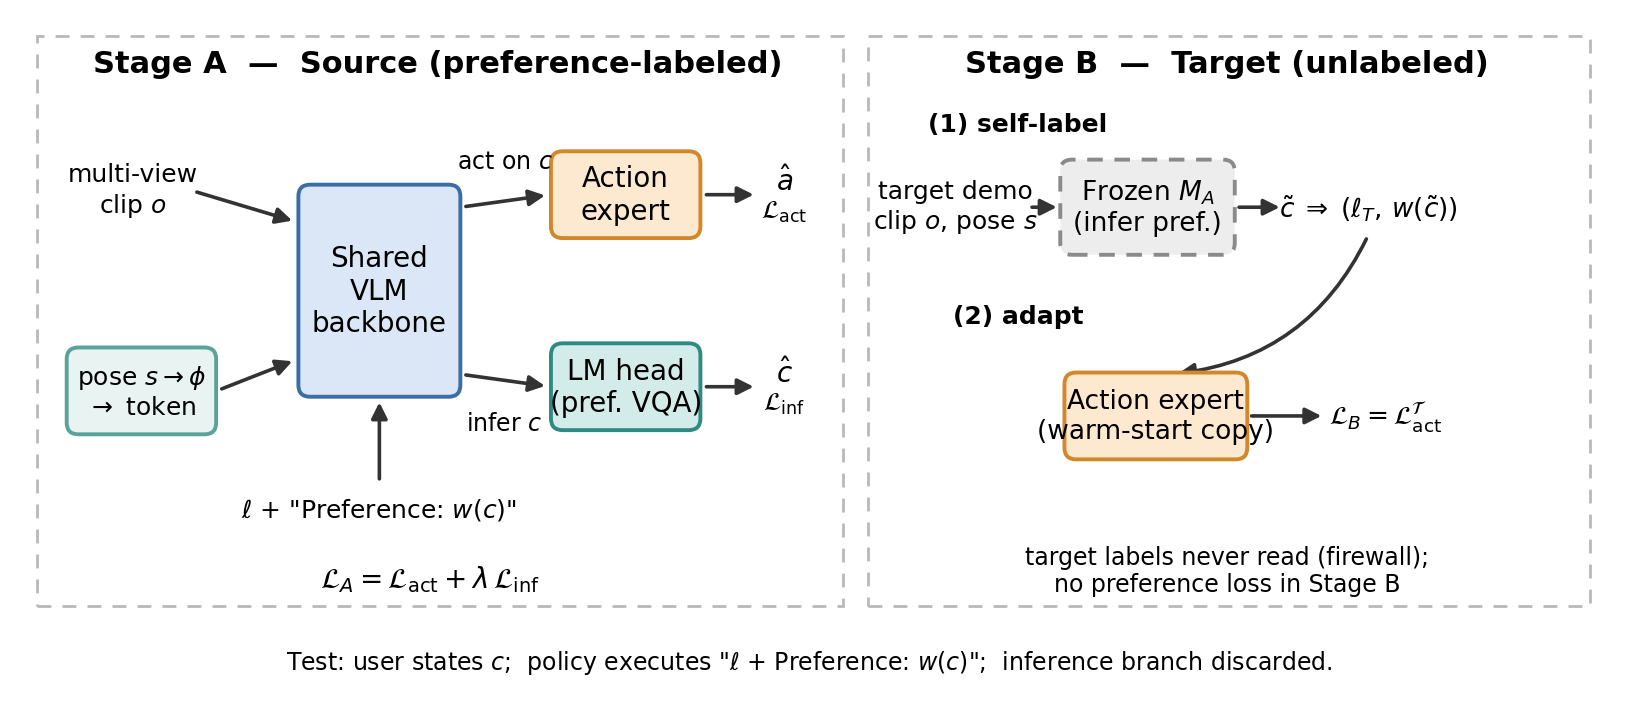
\includegraphics[width=\linewidth]{figures/method.png}
  \caption{\textbf{SPT} overview. One shared VLM
  backbone serves as a policy that acts on a stated preference (\emph{act on
  $c$}) and as a head that predicts the preference of a demonstration
  (\emph{infer $c$}). The prediction head reads the VLM's language output, and
  takes the proprioceptive state as a learned token $\phi(s)$. Stage~A trains
  both on the labeled source. Stage~B freezes this model, labels each unlabeled
  target demonstration with the prediction head, and continues training the
  action expert on the labeled prompts. At test time the user sets $c$ and only
  the policy is used.}
  \label{fig:method}
\end{figure}

\section{Problem Formulation}
\label{sec:formulation}

We consider a robot that performs manipulation tasks specified by natural language instructions.
Each task admits multiple valid solutions that vary along axes we call \emph{preferences}---dimensions such as grasp height, placement gentleness, or trajectory clearance that affect how the task is executed without changing what is accomplished.
Formally, a robot performs tasks named by a language instruction $\ell$, and along a given preference axis the task admits several acceptable executions, where the each axis is discretized into a finite vocabulary $\mathcal{C}$ of preference values (e.g., $\mathcal{C}=\{\mathrm{low},\mathrm{high}\}$ for grasp height), which serves as the interface through which users customize policy behavior at deployment.
  A demonstration is a trajectory $\xi=\{(o_t,s_t,a_t)\}_{t=1}^{T}$ of multi-view observations $o_t$, proprioceptive state $s_t$, and actions $a_t$, executed under some preference $c\in\mathcal{C}$.


Our goal is to transfer preference-following capabilities from a labeled source domain to an unlabeled target domain.
We are given two disjoint task sets that share the same preference vocabulary $\mathcal{C}$: a \emph{source} $\mathcal{S}$ that is densely preference-labeled, and a \emph{target} $\mathcal{T}$ that is not.
The source dataset $\mathcal{D}_{\mathcal{S}}=\{(\xi_{\mathcal{S}}^{(i)},\ell_{\mathcal{S}}^{(i)},c^{(i)})\}$ pairs every demonstration with both its instruction $\ell^{(i)}$ and its preference label $c^{(i)}$.
The target dataset $\mathcal{D}_{\mathcal{T}}=\{(\xi_{\mathcal{T}}^{(j)},\ell_{\mathcal{T}}^{(j)})\}$ carries no preference labels: each episode was executed under some $c\in\mathcal{C}$, but which value is unknown at training time.
Because $\mathcal{C}$ is shared across domains, a user can steer target tasks using the same vocabulary employed to label the source.

We aim to train a preference-conditioned policy $\pi_{\theta}(a\mid o,s,\ell,c)$ that, when deployed on a target task with a user-specified $c\in\mathcal{C}$, produces behavior consistent with that preference.
A rollout \emph{follows} preference $c$ when a per-axis criterion $\phi(\xi)$ matches the value designated by $c$---a threshold on continuous axes (e.g., minimum grasp contact height, obstacle clearance distance) or a discrete match on categorical axes (e.g., grasp orientation, strike strategy).
The central challenge is that $\mathcal{T}$ provides only $(\xi_\mathcal{T},\ell_\mathcal{T})$ pairs, not the preference-labeled prompts $(\ell_\mathcal{T},c)$ necessary to learn a mapping from preference specifications to behaviors on target tasks.
Preference-following on $\mathcal{T}$ must therefore be inherited from $\mathcal{S}$ through the model's internal understanding of preferences, without any direct supervision on the target.

\section{Methods}
\label{sec:methods}



As shown in Fig.~\ref{fig:method}, Self-Labeled Preference Transfer (SPT) trains the VLA in Stage~A both to act on a stated preference and to infer the preference from a demonstration, whose pre-trained backbone can then label the preferences of the target demonstrations in Stage~B.


\textbf{Architecture.}
\textcolor{red}{too complex/ detailed in description, do that part in the formulation instead here}
  For a VLA model, SPT initializes an extra head upon the shared VL-backbone in parallel to the action expert. 
  The backbone is a pretrained vision--language model (VLM) that encodes the multi-view observation, the proprioceptive state, and the text prompt. 
  An action expert decodes the backbone features into an action chunk; 
  we condition it on the preference through language, appending ``Preference:~$w(c)$'' to the instruction~$\ell$, where $w(c)$ is a fixed short
  phrase for each preference value (\eg, ``grasp low''). 
  For preference prediction we add no new module: we pose a binary question about the preference and read the answer off the VLM's language head as a single token. 
  Because both roles read the same backbone, training the predictor also shapes the features the policy uses.

  A preference is expressed mainly in how the robot moves, and is often only weakly visible in the camera views, which the model tends to ignore. Therefore, to augment the role of robot states, we applies a small MLP $\phi$ that encodes the end-effector pose \textcolor{red}{over the clip} into one token, which we insert into the VLM input next to the image tokens. 
  % The conditioning phrase $w(c)$ and the answer token may differ in surface form (, near/ far for the question, narrow/wide for the prompt), as long as both are fixed. [It is extremely hard to follow]

\textbf{Stage~A: joint source pretraining.}
On the densely-labeled source task set we co-train both directions, whose training batch mixes two sample types:
\emph{Action} samples pair an observation with its demonstrated action chunk under the preference prompt $(\ell, w(c))$, incurring an action-regression loss $\mathcal{L}_{\mathrm{act}}$;
\emph{Inference} samples pair a short demonstration clip (with its proprioceptive token) with the binary preference question, incurring a single-token cross-entropy loss $\mathcal{L}_{\mathrm{inf}}$. 
The resulting objective is as follows:
\begin{equation}
  \mathcal{L}_{A} \;=\; \mathcal{L}_{\mathrm{act}} \;+\; \lambda\,\mathcal{L}_{\mathrm{inf}},
  \label{eq:stageA}
\end{equation}
where $\lambda$ balances the two terms. This yields a source model $M_A=(\pi_{\theta_A},\,g_{\theta_A})$ whose policy $\pi_{\theta_A}$ executes preferences and whose inference branch $g_{\theta_A}$ identifies them.

\textbf{Stage~B: adaptation to the unlabeled target.}
We initialize from $M_A$ and adapt to the target task set using only its unlabeled demonstrations $\mathcal{D}_{\mathcal{T}}$, in two phases.
First, we \emph{self-label} the target by querying the \emph{frozen} source inference branch once per target episode,
\begin{equation}
  \tilde{c}^{(j)} \;=\; \arg\max_{c\in\mathcal{C}}\; g_{\theta_A}\!\big(c \mid o^{(j)},s^{(j)}\big).
  \label{eq:pseudolabel}
\end{equation}
This reconstructs the missing preference annotations as $(\ell_T,\tilde{c})$ pairs
that mirror the source format; the target's latent ground-truth preference is
never read at any point, so the ``unlabeled'' setting is preserved.
Second, we \emph{adapt}: starting from a warm-started copy of $M_A$, we continue
training the action expert on the self-labeled, preference-conditioned target
prompts, with the action loss alone,
\begin{equation}
  \mathcal{L}_{B} \;=\; \mathcal{L}^{\mathcal{T}}_{\mathrm{act}}\!\big(w(\tilde{c})\big).
  \label{eq:stageB}
\end{equation}
No ground-truth target preference is used, and the inference branch is not
  updated; the model bootstraps from its own source-trained understanding.

\textbf{Deployment.}
At test time on a target task, the user specifies the desired preference
$c\in\mathcal{C}$ from the source vocabulary, and the policy generates actions
conditioned on ``$\ell$.~Preference:~$w(c)$'', producing behavior in the
requested execution style. The inference branch is no longer needed and can be
discarded, leaving a standard preference-conditioned policy.




\section{Experiments}
\label{sec:experiments}

With experiments in simulation and on a real robot, and aim to answer two questions:
(i)~Does the preference prediction in SPT learned on the source transfer to the target,
that is, can the frozen source model label target demonstrations correctly?
(ii)~Does Stage~B in SPT turn those labels into a policy that follows the commanded
preference on the target?

\subsection{Experimental Setup}
\label{sec:setup}

\begin{figure}[t]
  \centering
  \includegraphics[width=\linewidth]{figures/sim.png}
    \caption{\textbf{Simulation Experiment Setup.} The base instruction is ``Pick up \textit{{A}} and place it on \textit{{B}}", where \textit{A} and \textit{B} denote different objects. Each column illustrates one preference type, while the two rows correspond to different preference values within that type. The preference types are: \textit{Grasp Contact Height}, \textit{Grasp Orientation}, \textit{Placement Location}, \textit{Obstacle Clearance}, and \textit{Release Height}. The commanded preference is highlighted in red, with the gray box indicating the corresponding preference value for each example.}
  \label{fig:sim}
\end{figure}


\begin{figure}[t]
  \centering
  \includegraphics[width=\linewidth]{figures/real.png}
  \caption{\textbf{Real-robot Experiment Setup.} We study two preference types: \textit{Obstacle Clearance} (left two columns) and \textit{Strike Strategy} (right two columns). For each preference type, the source task is shown in the first column and the unseen target task in the second column. The top and bottom rows correspond to the two preference values: \emph{short} and \emph{large} detours for obstacle clearance, and \emph{direct} and \emph{bank} shots for strike strategy. Red dashed lines indicate the preference-conditioned trajectories.}
  \label{fig:real}
\end{figure}


\textbf{Simulation benchmark.}
We synthesize a preference-varied manipulation dataset in RoboTwin~2.0~\citep{robotwin}, spanning five preference axes: \emph{grasp contact height} (low vs.\ high relative to the object), \emph{release height} (low vs.\ high above the target area), \emph{obstacle clearance} (narrow vs.\ wide detour when avoiding the obstacle), \emph{grasp orientation} (side vs.\ top), and \emph{placement location} (center vs.\ corner).
For each axis the source has 8 tasks, each demonstrated under both preference values with 100 demonstrations per value. 
The target is a held-out task with new objects on the same axis, whose instructions do not contain the preference for naive preference-following fine-tuning. 
% Observations are three Intel RealSense~L515 RGB views.

\textcolor{red}{Use less () if possible}
\textbf{Real-robot validation.}
We test on a UR5e under two cross-task settings. 
For \emph{obstacle clearance}, we label a near vs.\ far clearance preference on pick-and-place and transfer it to pushing (push a bowl around an obstacle). 
For \emph{strike strategy}, we label a direct vs.\ bank-shot preference on air hockey and transfer it to billiards (cue the ball into a pocket directly or off a cushion). Same as the simulation setup, the preference instructions are not included on the targeted task. 
Each target shares the source axis but differs in objects, dynamics, and goal. \textcolor{red}{Word target is overload here, change that if possible}

\textbf{Metrics.}
To evaluate the performance of label-free preference transfer, we consider 3 metrics:
\begin{itemize}
    \item \textbf{Recognition Accuracy.} is how often the frozen source predictor assigns the correct preference to a target demonstration compared with random guess (50\%).
    \item \textbf{Preference-following Accuracy.} is the fraction of rollouts whose behavior matches the commanded preference, scored by a per-axis statistic $\phi$, with continuous axes thresholded from source statistics and categorical axes matched directly. 
    \item \textbf{Task Success.} is the completion rate regardless of preference-following accuracy.
\end{itemize}

\textbf{Baseline.}
Our baseline is \emph{Naive FT}: starting from the same warm-started backbone as
SPT, we finetune on all available demonstrations with the action loss only, the
preference-labeled source under its preference prompt and the unlabeled target
under its instruction alone. It uses neither the Stage-A recognition objective
nor the Stage-B self-labels, so on the target nothing ties the executed motion to
a preference value. This isolates the effect of SPT's two ingredients while
holding the backbone, data, and compute budget fixed.








\textbf{Implementation details.}
The backbone is Qwen3-VL-4B. 
The action expert is an action-token head in the OpenVLA-OFT style, trained with an $L_1$ loss on $14$-D joint action chunks of horizon $50$, and warm-started from a manipulation-pretrained checkpoint. 
The prediction head is the VLM's language head, supervised with single-token cross-entropy over a short head-camera clip. 
We encode the active end-effector pose at the clip frames with a small MLP $\phi$ ($9\!\to\!512\!\to\!h$) and inject it as a token at an existing special-token slot, so the pretrained checkpoint loads without resizing the embedding. 
Stage~A optimizes $\mathcal{L}_A$; Stage~B continues training the action expert at a lower learning rate.  and the $\phi$ and $w(\cdot)$ vocabularies.


\begin{table}[t]
  \centering
  \small
  \caption{\textbf{Prediction transfer (simulation).} Accuracy of the frozen
  source predictor on the target, per preference axis (chance $=50\%$). It
  depends only on the Stage-A predictor, so it is reported once per axis.}
  \label{tab:sim_recognition}
  \begin{tabular}{lc}
    \hline
    Preference axis & Recognition Acc.\ (\%) \\
    \hline
    Grasp contact height & 100 \\
    Release height       & 100 \\
    Obstacle clearance   & 92 \\
    Grasp orientation    & 100 \\
    Placement location   & 90 \\
    \hline
    Average              & 96.4 \\
    \hline
  \end{tabular}
\end{table}

\begin{table}[t]
  \centering
  \small
  \caption{\textbf{Preference-following and task success (simulation).} Per-axis
  results for SPT and the Naive FT baseline.}
  \label{tab:sim_main}
  \begin{tabular}{lcccc}
    \hline
    & \multicolumn{2}{c}{Following Acc.\ (\%)} & \multicolumn{2}{c}{Success (\%)} \\
    Preference axis & Naive FT & SPT & Naive FT & SPT \\
    \hline
    Grasp contact height & 59 & 90 & 92 & 95 \\
    Release height       & 53 & 81 & 89 & 91 \\
    Obstacle clearance   & 57 & 75 & 85 & 82 \\
    Grasp orientation    & 61 & 95 & 94 & 92 \\
    Placement location   & 67 & 83 & 80 & 86 \\
    \hline
    Average              & 59.4 & \textbf{84.8} & 88 & 89.2 \\
    \hline
  \end{tabular}
\end{table}

\begin{table}[t]
  \centering
  \small
  \caption{\textbf{Real-robot results (UR5e).} Preference-following accuracy and
  task success on two cross-task settings, SPT vs.\ Naive FT. }
  \label{tab:real_main}
  \begin{tabular}{llccccc}
    \hline
    & & \multicolumn{2}{c}{Following Pref. Rate\ } & \multicolumn{2}{c}{Success Rate} \\
    Setting & Preference & Naive FT & SPT & Naive FT & SPT \\
    \hline
    Obstacle clearance & near    & 6/10 & 10/10 & 9/10 & 10/10 \\
    (push)             & far     & 5/10 & 10/10 & 10/10 & 10/10 \\
    Strike strategy    & direct  & 5/10 & 9/10 & 8/10 & 8/10 \\
    (billiards)        & bank    & 5/10 & 8/10 & 9/10 & 10/10 \\
    \hline
  \end{tabular}
\end{table}

\subsection{Main Results}
\label{sec:exp-main}

\textbf{Preference prediction transfers to the target.}
Table~\ref{tab:sim_recognition} reports the frozen predictor's accuracy on the
target, per axis. It is well above the $50\%$ chance line on all five axes
(96.4\% on average, and at least 90\% on every axis). Three axes---grasp contact
height, release height, and grasp orientation---reach a perfect 100\%: here the
preference is carried by a single distinctive end-effector height or pose, which
the proprioceptive token $\phi(s)$ exposes to the predictor directly. The two
lowest, placement location (90\%) and obstacle clearance (92\%), are the more
\emph{relational} axes, where the preference surfaces in the object's final
location or in the shape of the detour path rather than in one arm pose. Even on
the hardest axis the predictor errs on only one demonstration in ten, and fewer
than 4\% of self-labels are wrong on average, so the labels Stage~B trains on are
nearly noise-free. Because these predictions \emph{are} the supervision Stage~B
consumes, their quality upper-bounds what the policy can learn---a link we see
borne out below.

\textbf{SPT follows the commanded preference, while Naive FT ignores it.}
Table~\ref{tab:sim_main} reports preference-following and success in simulation
and Table~\ref{tab:real_main} on the UR5e. Naive FT follows the prompt in only
53--67\% of simulated rollouts (59.4\% on average) and 52.5\% on the real
robot---barely above the 50\% chance line---yet still completes the task at
80--94\% in simulation and 8--10 of 10 on the robot. It is a competent but
\emph{single-minded} policy: lacking any link between the prompt and the
demonstrated motion, it settles on one dominant mode and is insensitive to the
preference. SPT removes exactly this failure. It lifts following to 84.8\% in
simulation (a 25.4-point gain) and to 92.5\% on the real robot (a roughly
40-point gain), with per-axis simulation gains ranging from +16 points (placement
location) to +34 (grasp orientation). The gap is widest on the real robot, where
the target differs from the source in objects, dynamics, and goal: Naive FT
collapses to chance, whereas SPT reaches 10/10 on both push-clearance preferences
and 8--9/10 on the two billiards strike strategies.

\textbf{Following gains track recognition, and come at no cost to success.}
Two patterns cut across the axes. First, SPT's gains are largest where the
preference is a clean, pose-separable signal---grasp orientation (+34) and grasp
contact height (+31)---and smallest on the two relational axes, placement location
(+16) and obstacle clearance (+18), precisely the axes where recognition is
weakest; following quality tracks self-label quality, as expected when Stage~B is
trained on those self-labels. Second, this added steerability is essentially free:
SPT's task success is statistically flat against Naive FT (89.2\% vs.\ 88\% on
average in simulation, and matching or exceeding it on all four real-robot
conditions), rising on three simulated axes and dipping by at most three points on
the other two. Following the commanded preference therefore does not trade off
against completing the task---SPT supplies the missing steerability while
preserving the competence the baseline already had. 








% \begin{table}[t]
%   \centering
%   \small
%   \caption{\textbf{Ablation of SPT's two components} (simulation, averaged over
%   the five axes). \textbf{PL}: Stage-B self-label conditioning only;
%   \textbf{VQA}: Stage-A prediction loss only; \textbf{SPT}\,=\,both
%   (Section~\ref{sec:exp-setup}).}
%   \label{tab:ablation}
%   \begin{tabular}{lcc}
%     \hline
%     Configuration & Following Acc.\ (\%) & Success (\%) \\
%     \hline
%     B0 \,(neither)              & -- & -- \\
%     PL \,(conditioning only)    & -- & -- \\
%     VQA (prediction only)       & -- & -- \\
%     SPT (both)                  & \textbf{--} & -- \\
%     \hline
%   \end{tabular}
% \end{table}

\section{Conclusion and Discussion}
\label{sec:conclusion_discussion}

\subsection{Conclusion}
\label{sec:conclusion}

We started from a single observation: training a vision-language backbone on densely labeled source preferences does two jobs at once---it shapes a representation the action head can \emph{steer} from a stated preference, and it teaches the backbone to \emph{read} the preference back out of a demonstration. This addresses \emph{label-free preference transfer}, where preferences are densely labeled on a source task set and must be inherited on a target set that supplies demonstrations but no labels, so that the upfront labeling investment amortizes across future tasks rather than recurring for each one. \textbf{Self-Labeled Preference Transfer (SPT)} turns this coupling into a transfer recipe: Stage~A co-trains a preference-conditioned action expert and a single-token preference-recognition head over one shared backbone, and Stage~B reuses that frozen backbone as a self-labeler to supply the missing target preferences, then continues training only the action expert on the resulting preference-conditioned prompts---without any target annotation. Across five preference axes in simulation, the frozen source predictor labels the target with \textbf{96.4\%} accuracy and at least \textbf{90\%} on every axis, and SPT raises preference-following to \textbf{84.8\%} from the Naive~FT baseline's \textbf{59.4\%}, a \textbf{25.4}-point gain, while task success is essentially unchanged (\textbf{89.2\%} vs.\ \textbf{88\%}). On a real UR5e, the same recipe transfers preference control to two unlabeled tasks the policy never saw labeled, pushing and billiards, lifting preference-following from a near-chance \textbf{52.5\%} to \textbf{92.5\%} without sacrificing task completion. By making preference-following a capability that transfers like task, scene, and object understanding, SPT recovers on unlabeled tasks the steerability that naive finetuning washes out, and turns preference customization from a per-task annotation cost into a transferable property of VLAs.

\subsection{Limitations and Future Work}
\label{sec:limitations}

SPT inherits the source preference set $\mathcal{C}$: a user can steer the target only with values defined and labeled on the source, so a new value on an axis, a whole new axis, or continuous control at test time is out of scope. It is further bounded by its own self-labels---Stage~B trains the action expert on the frozen predictor's outputs alone, so its ceiling is the recognition accuracy, which is weakest on the more relational axes (placement location, obstacle clearance) where the preference lives in the object's final location or detour path rather than a single arm pose, and the predictor never abstains, silently mapping out-of-vocabulary behavior to the nearest source value. Extending the vocabulary to new or continuous values, composing labeled axes, and discovering preference axes from data are left to future work.









% ============================ FIGURES ================================

% \begin{figure}[t]
%   \centering
%   % \includegraphics[width=\linewidth]{figures/real_overlay.pdf}
%   \framebox[\linewidth]{\begin{minipage}{0.95\linewidth}\centering\vspace{2.2cm}
%     \textit{[Figure placeholder] Top-down trajectory overlays on the real robot. Left: clearance setting, near vs.\ far around the candle, SPT vs.\ B0. Right: strike setting, direct vs.\ bank in billiards, SPT vs.\ B0.}
%     \vspace{2.2cm}\end{minipage}}
%   \caption{\textbf{Real-robot trajectory overlays.} On unlabeled target tasks, SPT produces distinct trajectories for the two commanded preferences (hug vs.\ swing wide; direct vs.\ bank), while B0 is insensitive to the prompt.}
%   \label{fig:real_overlay}
% \end{figure}

% \begin{figure}[t]
%   \centering
%   % \includegraphics[width=\linewidth]{figures/sim_dist.pdf}
%   \framebox[\linewidth]{\begin{minipage}{0.95\linewidth}\centering\vspace{1.8cm}
%     \textit{[Figure placeholder] Distribution of the per-axis statistic phi under the low vs.\ high prompt on the unlabeled target, SPT vs.\ B0, per axis.}
%     \vspace{1.8cm}\end{minipage}}
%   \caption{\textbf{Preference-following in simulation.} Under opposite commanded preferences, SPT shifts the executed statistic $\phi$ to opposite sides of the threshold; B0 does not separate.}
%   \label{fig:sim_dist}
% \end{figure}



\clearpage
% The acknowledgments are automatically included only in the final and preprint versions of the paper.


%===============================================================================

% no \bibliographystyle is required, since the corl style is automatically used.
\bibliography{example}  % .bib

\end{document}
